\documentclass{standalone}
\usepackage{tikz}

% == Tikz
\newcommand{\drawcirc}{\node[draw,circle,minimum size=1.5cm]}
\newcommand{\drawcircred}{\node[red, draw,circle,minimum size=1.5cm]}
\newcommand{\drawbox}{\node[draw,rectangle,minimum size=1.5cm]}
\newcommand{\drawboxred}{\node[red, draw,rectangle,minimum size=1.5cm]}
\newcommand{\drawdummy}{\node[minimum size=0,inner sep=0]}
\newcommand{\zeroSink}{\mathsf{o}}
\newcommand{\target}{\mathsf{f}}

\begin{document}
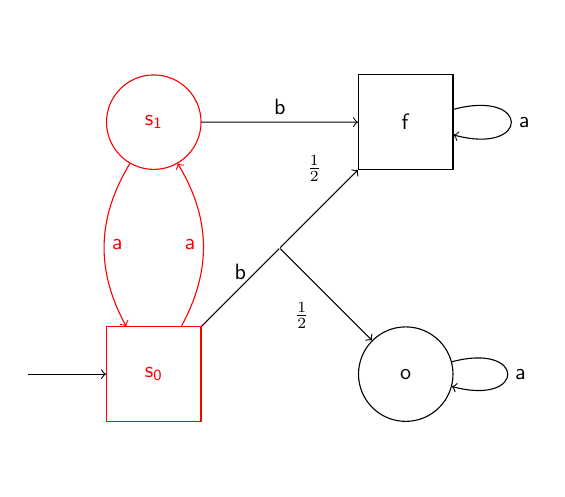
\begin{tikzpicture}[scale=0.8, every node/.style={transform shape}]
%little BCEC with loop
\drawdummy (init) at (-2,0) {};
\drawdummy (space1) at (0,5.5){};
\drawdummy (space2) at (0,-1.5){};
\drawboxred (q) at (0,0) {$\mathsf{s_0}$};
\drawcircred (p) at (0,4) {$\mathsf{s_1}$};
\drawdummy (mid) at (2,2) {};
\drawbox (1) at (4,4) {$\target$ };
\drawcirc (0) at (4,0)  {$\mathrm{\zeroSink}$};

\draw[->] (init) to (q);
\draw[red, ->]  (q) to [bend right] node [left ,midway] {$\mathsf{a}$}(p);
\draw[red, ->]  (p) to [bend right] node [right, midway] {$\mathsf{a}$}(q);
\draw[->]  (p) to node [midway,anchor=south] {$\mathsf{b}$}(1) ;
\draw[-] (q) to node [midway,anchor=south] {$\mathsf{b}$} (mid) ;
\draw[->] (mid) to node [text width =1.0cm, midway, below] {$\frac{1}{2}$} (0);
\draw[->] (mid) to node [text width =1.0cm, near end, above] {$\frac{1}{2}$} (1);
%\draw (mid) to [bend left,out=270,in=270] (q) ;
\draw[->]  (0) to[loop right]  node [midway,right] {$\mathsf{a}$} (0);
\draw[->]  (1) to [loop right] node [midway,right] {$\mathsf{a}$} (1);
\end{tikzpicture}
\end{document}
